\documentclass[aspectratio=169]{beamer}

\usepackage{amsmath}
\usepackage{graphicx}
\usepackage{tikz}
\usetikzlibrary{arrows.meta,positioning,shapes.geometric,calc}

\setbeamertemplate{navigation symbols}{}
\setbeamertemplate{footline}[frame number]
\setbeamertemplate{frametitle}{
  \vspace{0.4em}
  \insertframetitle\par
  \vspace{0.3em}
  \hrule
}

\setbeamercolor{background canvas}{bg=white}
\setbeamercolor{normal text}{fg=black,bg=white}
\setbeamercolor{frametitle}{fg=black,bg=white}
\setbeamercolor{title}{fg=black}
\setbeamercolor{subtitle}{fg=black}

\title{A 46 $\mu$W 13 b 6.4 MS/s SAR ADC\\with Background Mismatch and Offset Calibration}
\subtitle{Pieter Harpe et al.\\IEEE JSSC, 2017}
\author{Jesse Levine}
\date{}

\definecolor{linegray}{RGB}{120,120,120}
\definecolor{softgray}{RGB}{245,245,245}
\definecolor{softblue}{RGB}{233,242,252}
\definecolor{softgreen}{RGB}{235,248,238}
\definecolor{softred}{RGB}{252,239,239}

\tikzset{
  box/.style={
    draw=linegray,
    rounded corners=1.5mm,
    thick,
    align=center,
    fill=softgray,
    inner sep=5pt,
    font=\small
  },
  flow/.style={-Latex, thick, draw=black}
}

\begin{document}

\begin{frame}
  \begin{columns}[T]
    \begin{column}{0.56\textwidth}
      \vspace{1.1cm}
      \centering
      {\LARGE \inserttitle \par}
      \vspace{0.45cm}
      {\large \insertsubtitle \par}
      \vspace{1.0cm}
      {\large ELEC5705 \par}
      \vspace{0.25cm}
      {\large \insertauthor \par}
    \end{column}
    \begin{column}{0.44\textwidth}
      \centering
      
\includegraphics[width=\linewidth]{Figures/Paper_title.png}

      \vspace{2mm}

      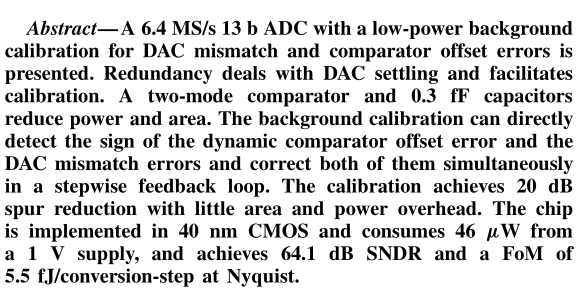
\includegraphics[width=\linewidth]{Figures/Paper_abstract.png}
    \end{column}
  \end{columns}
\end{frame}

\begin{frame}{Introduction}
  \begin{columns}[T]
    \begin{column}{0.62\textwidth}
      \scriptsize
      \begin{itemize}
        \item Wireless standards such as \textbf{IEEE 802.15.4g} need \textbf{high-resolution} ADCs at MS/s rates with \textbf{very low power}.
        \item SAR ADCs are attractive because they are already very \textbf{energy efficient}.
        \item Above roughly \textbf{10 bits}, the main limits become \textbf{DAC mismatch} and \textbf{noise / comparator offset}.
        \item Larger capacitors improve matching, but hurt \textbf{power}, \textbf{area}, and \textbf{speed}.
        \item Prior fixes such as \textbf{DSP/LMS}, \textbf{statistics-based methods}, pipelined SAR + amplifier, or comparator oversampling all add overhead.
        \item This paper instead proposes a \textbf{13-bit SAR ADC} with a \textbf{reconfigurable comparator} and \textbf{low-power background calibration} for DAC mismatch and dynamic comparator offset.
      \end{itemize}
    \end{column}
    \begin{column}{0.38\textwidth}
      \centering
      \scriptsize
      \begin{tabular}{|l|c|}
        \hline
        \multicolumn{2}{|c|}{\textbf{Reported results}} \\
        \hline
        Resolution & 13 b \\
        \hline
        Sampling rate & 6.4 MS/s \\
        \hline
        Power & 46 $\mu$W \\
        \hline
        ENOB & 10.4 b \\
        \hline
        SNDR & 64.1 dB \\
        \hline
        FoM & 5.5 fJ/conv-step \\
        \hline
      \end{tabular}
    \end{column}
  \end{columns}
\end{frame}

\begin{frame}{Design Philosophy}
  \begin{columns}[T]
    \begin{column}{0.56\textwidth}
      \small
      \begin{itemize}
        \item \textbf{Minimalist calibration}: do the least computation needed for the maximum return.
        \item Do \textbf{not} estimate full error magnitude with heavy DSP.
        \item Detect only the \textbf{sign / direction} of the error.
        \item Let a lightweight controller repeatedly nudge the hardware in the right direction.
        \item Result: an elegant, low-overhead \textbf{closed-loop control system} inside the SAR ADC.
      \end{itemize}
    \end{column}
    \begin{column}{0.44\textwidth}
      \centering
      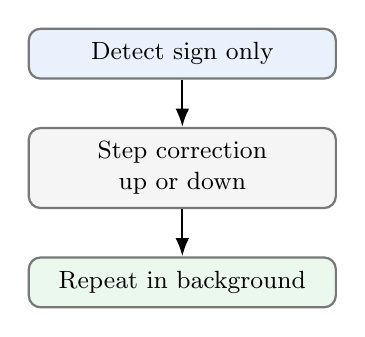
\begin{tikzpicture}[node distance=6mm]
        \node[box, fill=softblue, minimum width=3.9cm] (obs) {Detect sign only};
        \node[box, fill=softgray, below=of obs, minimum width=3.9cm] (step) {Step correction\\up or down};
        \node[box, fill=softgreen, below=of step, minimum width=3.9cm] (repeat) {Repeat in background};
        \draw[flow] (obs) -- (step);
        \draw[flow] (step) -- (repeat);
      \end{tikzpicture}
    \end{column}
  \end{columns}
\end{frame}

\begin{frame}{Architecture and Closed-Loop Idea}
  \small
  \centering
  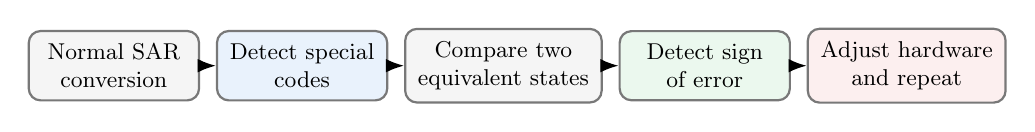
\begin{tikzpicture}[node distance=2.2mm, scale=0.92, transform shape]
    \node[box, fill=softgray, minimum width=2.35cm, minimum height=0.8cm] (n1) {Normal SAR\\conversion};
    \node[box, fill=softblue, right=of n1, minimum width=2.35cm, minimum height=0.8cm] (n2) {Detect special\\codes};
    \node[box, fill=softgray, right=of n2, minimum width=2.35cm, minimum height=0.8cm] (n3) {Compare two\\equivalent states};
    \node[box, fill=softgreen, right=of n3, minimum width=2.35cm, minimum height=0.8cm] (n4) {Detect sign\\of error};
    \node[box, fill=softred, right=of n4, minimum width=2.35cm, minimum height=0.8cm] (n5) {Adjust hardware\\and repeat};
    \draw[flow] (n1) -- (n2);
    \draw[flow] (n2) -- (n3);
    \draw[flow] (n3) -- (n4);
    \draw[flow] (n4) -- (n5);
  \end{tikzpicture}

  \vspace{3mm}

  \begin{columns}[T]
    \begin{column}{0.46\textwidth}
      \small
      \begin{itemize}
        \item Standard differential SAR ADC with \textbf{monotonic switching}.
        \item Uses \textbf{15 comparison cycles} for a \textbf{13-bit} conversion.
        \item Two \textbf{redundant cycles} make calibration observable and tolerate DAC settling / comparator error.
        \item An optional \textbf{16th cycle} is inserted only for calibration.
        \item Final output is computed from the \textbf{15-bit raw code}.
      \end{itemize}
    \end{column}
    \begin{column}{0.54\textwidth}
      \centering
      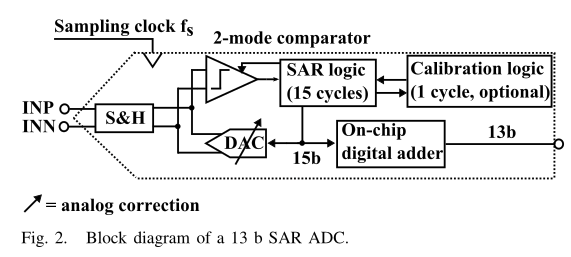
\includegraphics[width=\linewidth]{Figures/Figure2.png}
    \end{column}
  \end{columns}
\end{frame}

\begin{frame}{Digital Side: Lightweight Controller}
  \begin{columns}[T]
    \begin{column}{0.56\textwidth}
      \scriptsize
      \textbf{1. Sense \& Force trigger logic}
      \begin{itemize}
        \item Monitor specific internal SAR codes during the normal \textbf{15-cycle} conversion.
        \item Implemented with \textbf{dynamic logic}; effectively ``asleep'' about \textbf{90\%} of the time.
      \end{itemize}

      \textbf{2. Extra 16th cycle}
      \begin{itemize}
        \item If a trigger code appears, the controller inserts an extra \textbf{16th cycle}.
        \item \textbf{DAC mismatch}: compare two redundant codes \(A\) and \(B\) that should produce the same voltage.
        \item \textbf{Comparator offset}: compare fine mode and coarse mode with the DAC code held constant.
      \end{itemize}

      \textbf{3. Sign detection and filtering}
      \begin{itemize}
        \item Compare \(D_{15}\) and \(D_{16}\) to get only the \textbf{sign} of the error.
        \item Feed that sign to a \textbf{6-bit bidirectional-counter} LPF.
        \item Only when a counter reaches \textbf{0 or 63} does the analog calibration register update.
      \end{itemize}

    \end{column}
    \begin{column}{0.44\textwidth}
      \centering
      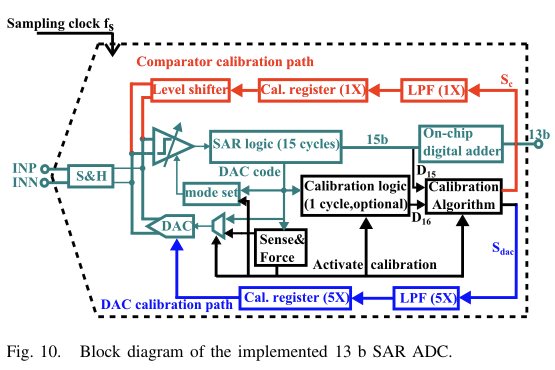
\includegraphics[width=0.88\linewidth]{Figures/Figure10.png}
    \end{column}
  \end{columns}
\end{frame}

\begin{frame}{Analog Side: Physical Error Correction}
  \begin{columns}[T]
    \begin{column}{0.50\textwidth}
      \scriptsize
      \textbf{DAC mismatch correction}
      \begin{itemize}
        \item Only the \textbf{top 5 MSB capacitors} are calibrated.
        \item Each has a programmable bank of tiny \textbf{75 aF} trim capacitors.
        \item These implement \textbf{0.25 LSB} correction steps by adding or subtracting capacitance from the main DAC bit weight.
      \end{itemize}

      \textbf{Comparator offset correction}
      \begin{itemize}
        \item A \textbf{2-mode comparator} saves power but creates a dynamic offset shift.
        \item Two programmable capacitor banks, \(C_a\) and \(C_b\), inject a small compensating input step.
        \item Digital logic only chooses the control word; the actual correction happens \textbf{in analog}.
      \end{itemize}

      \vspace{1mm}
      \textbf{Key point:} the digital side decides \emph{when} and \emph{which direction}; the analog side performs the actual fix.
    \end{column}
    \begin{column}{0.50\textwidth}
      \centering
      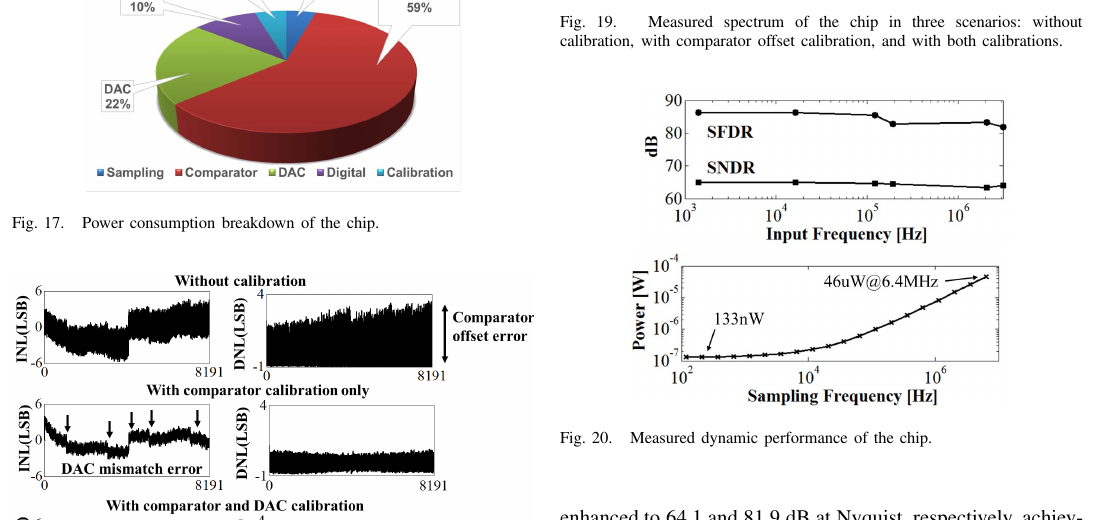
\includegraphics[width=0.80\linewidth]{Figures/Figure13_crop.png}

      \vspace{1mm}

      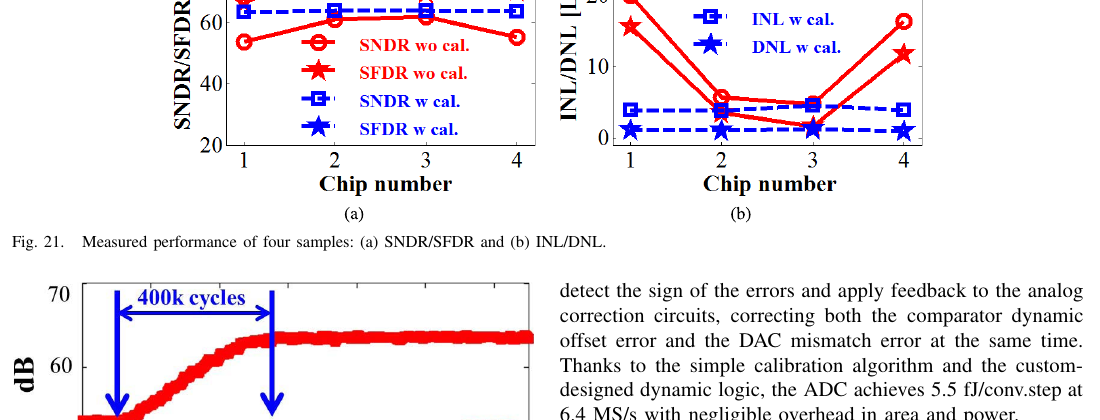
\includegraphics[width=0.80\linewidth]{Figures/Figure14_crop.png}
    \end{column}
  \end{columns}
\end{frame}

\begin{frame}{Measurements Summary}
  \centering
  \small
  \begin{tabular}{|l|c|}
    \hline
    \multicolumn{2}{|c|}{\textbf{Measured / Reported Results}} \\
    \hline
    Process & 40 nm CMOS \\
    \hline
    Supply voltage & 1 V \\
    \hline
    Active area & 0.0675 mm$^2$ \\
    \hline
    Digital calibration area & 0.0017 mm$^2$ \\
    \hline
    Analog correction area & 0.0009 mm$^2$ \\
    \hline
    Sampling rate & 6.4 MS/s \\
    \hline
    Resolution & 13 b \\
    \hline
    Total power & 46 $\mu$W \\
    \hline
    Calibration power overhead & $\sim$5\% \\
    \hline
    ENOB & 10.4 b \\
    \hline
    SNDR & 64.1 dB \\
    \hline
    SFDR & 81.9 dB \\
    \hline
    FoM & 5.5 fJ/conv-step \\
    \hline
    Spur reduction from calibration & $\sim$20 dB \\
    \hline
    Convergence time & $\sim$400k cycles \\
    \hline
  \end{tabular}
\end{frame}

\end{document}
